\documentclass[tikz,border=5pt]{standalone}
\usepackage{amsmath}
\begin{document}
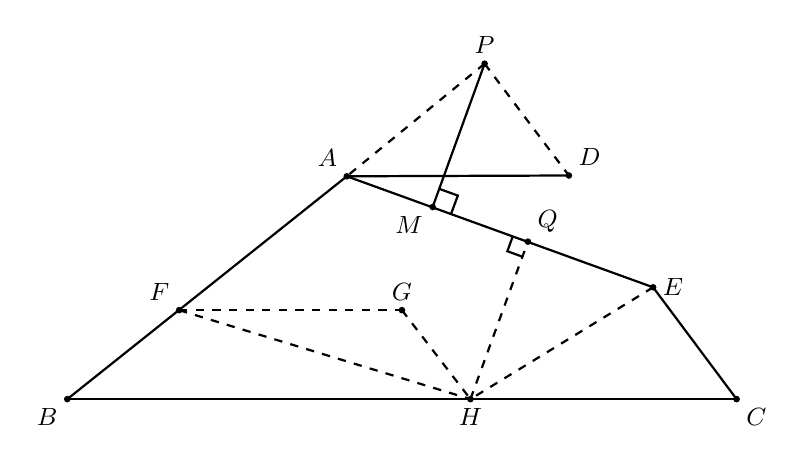
\begin{tikzpicture}[
  every node/.style={font=\small},
  dot/.style={circle, fill=black, inner sep=0.8pt}
]

% 坐标点
\coordinate (B) at (0,0);
\coordinate (C) at (8.5,0);
\coordinate (H) at (5.12,0);
\coordinate (A) at (3.55,2.83);
\coordinate (D) at (6.37,2.84);
\coordinate (E) at (7.44,1.42);
\coordinate (F) at (1.42,1.13);
\coordinate (G) at (4.25,1.13);
\coordinate (P) at (5.30,4.26);
\coordinate (Q) at (5.85,2.00);
\coordinate (M) at (4.64,2.44);

% 实线：三角形边 AB、BC、CE，以及 AD、AE（DE 段已删除）
\draw[solid, thick] (B) -- (A);
\draw[solid, thick] (B) -- (C);
\draw[solid, thick] (E) -- (C);
\draw[solid, thick] (A) -- (D);
\draw[solid, thick] (A) -- (E);

% 虚线：延长线与辅助线
\draw[dashed, thick] (P) -- (A);
\draw[dashed, thick] (P) -- (D);
\draw[dashed, thick] (F) -- (G);
\draw[dashed, thick] (F) -- (H);
\draw[dashed, thick] (G) -- (H);
\draw[dashed, thick] (E) -- (H);
\draw[dashed, thick] (H) -- (Q);

% 新增：从 P 向 AE 作垂线 PM
\draw[solid, thick] (P) -- (M);

% 垂足 M 处的直角标记
\draw[thick] (4.875,2.355) -- (4.96,2.585) -- (4.725,2.670);

% 垂足 Q 处的直角标记
\draw[thick] (5.657,2.066) -- (5.589,1.878) -- (5.777,1.810);

% 顶点与点标记
\node[below left] at (B) {$B$};
\node[below right] at (C) {$C$};
\node[below] at (H) {$H$};
\node[above left] at (A) {$A$};
\node[above right] at (D) {$D$};
\node[right] at (E) {$E$};
\node[above left] at (F) {$F$};
\node[above] at (G) {$G$};
\node[above] at (P) {$P$};
\node[above right] at (Q) {$Q$};
\node[below left] at (M) {$M$};

% 标记点（可选的小圆点）
\foreach \p in {A,B,C,D,E,F,G,H,P,M,Q}
  \fill (\p) circle (1.2pt);

\end{tikzpicture}
\end{document}
